\newcommand{\ignore}[1]{}
\subsubsection{\stid{3.07} Factorization Based Sparse Solvers and Preconditioners for Exascale} \label{subsubsect:strumpack}

\paragraph{Overview} 
% \textit{Provide an overview of your project.  You might find that the introductory text from your Fall 2017 Project Summary \url{https://confluence.exascaleproject.org/display/1ST/Fall+2017+ECP+ST+Project+Summaries} useful as a starting draft.}
In this project we will deliver factorization based sparse solvers
encompassing the two widely used algorithm variants: supernodal
(SuperLU library) and multifrontal (STRUMPACK library). STRUMPACK is
further enhanced with scalable preconditioning functionality using
hierarchical matrix algebra. Both libraries are purely algebraic,
applicable to a large variety of application domains. We will address
several challenges that arise in Exascale computing, with the following
focus areas: 
(1) Develop novel approximation algorithms that have lower
arithmetic and communication complexity with respect to the size of the
input matrix;
(2) Develop new parallelization strategies that reduce
inter-process communication and expose task parallelism and vectorization
for irregular computations involving sparse data structures to better
use on-node resources;
(3) Integrate our software into the higher level
algebraic solvers such as hypre, PETSc, Trilinos, and collaborate with
ECP application teams for application-specific and hardware-specific tuning
of the parameters space to achieve optimal efficiency of our solvers.

Our solver technology is essential for ECP, because many DOE simulation
and data analysis codes expected to run on the Exascale machines need
solutions of sparse algebraic systems, and many high fidelity simulations
involve large-scale multiphysics and multiscale modeling problems that
generate highly ill-conditioned and indefinite algebraic equations,
for which pure iterative methods such as Krylov and multigrid, albeit
readily parallelizable on large machines, cannot converge to the solution.
The factorization based algorithms being developed herein
represent an important class of methods that are indispensable building
blocks for solving those numerically challenging problems. Our software
can often be used as a reliable standalone solver, or as a preconditioner
for Krylov iterative methods, or as a coarse grid solver in multigrid
methods, just to name a few.

\paragraph{Key Challenges}
%\textit{Describe what is hard to do, why it is challenging.}
At Exascale we need to address several major challenges:
decreasing amount of memory per core, larger impact of communication
cost and load imbalance, more heterogeneous architecture.
Our new design of algorithms and codes need to focus on
reducing communication and synchronization and task scheduling 
instead of floating point operation throughput. In sparse factorization
methods, we expect new bottlenecks in parts of the code
that previously received little attention. For example, the preprocessing
step involves numerical pivoting for selecting stable pivots and
symbolic factorization, which do not yet parallelize well on manycore
architectures with fine-grained parallelism.
At Exascale, direct solvers are more likely to
be used in a preconditioning strategy, for example, in block Jacobi
preconditioning, in domain decomposition methods or as coarse-grid
solvers in algebraic multigrid, which requires repeated triangular
solves. The challenge here is to mitigate the low arithmetic intensity
and high degree of data dependency.

Compared to iterative methods, the primary bottleneck of direct solvers
is the asymptotically higher growth in memory need and floating point
operations, especially for problems from three-dimensional geometry.
It is imperative to develop novel factorization methods which require
much less memory footprint and data movement.


\paragraph{Solution Strategy}
%\textit{Describe your basic strategy for addressing the challenges.}
We will address these challenges in several thrust areas.
The new techniques will be implemented in the two software packages SuperLU
and STRUMPACK. The former is a widely used sparse direct solver based on
supernodal factorization and the latter is a newer direct
solver/preconditioner package based on multifrontal factorization 
and hierarchical low-rank matrix structures.
% Parallel pre-pivoting for both packages.

The improvements for SuperLU will be mainly in two areas: (1) develop
a communication-avoiding 3D factorization code that has provably 
lower communication complexity; (2) develop a synchronization-avoiding
triangular solve code to enable more overlap of communications of different
processes at different substitution steps.

In addition to exploiting structural sparsity as SuperLU does, STRUMPACK
also exploits data sparseness in the dense blocks of sparse factors using
low-rank representations, which leads to linear scaling $O(n)$ or $O(n \log n)$
memory and arithmetic complexity for PDEs with smooth kernels.
The developments for STRUMPACK will focus on several areas:
(1) develop robust stopping criteria --- both absolute and relative --- for
    adaptive (incremental) randomized sampling schemes to reveal numerical
    ranks in the low-rank compression routine. The goal is to use
    enough samples for stability, but not too many for efficiency;
(2) add OpenMP support for both HSS compression and ULV factorization routines,
    especially use OpenMP task construct to support irregular parallelism.
(3) reduce MPI communication in all stages of the code, including HSS
    construction, ULV factorization and triangular solve;
(4) in addition to HSS, develop codes to support other simpler low-rank
    formats, such as HOLDR. The HSS format has asymptotically lower complexity
    than HOLDR, but has a larger prefactor constant. We expect HSS to be more
    useful for large-scale problems while HOLDR is more useful for mid-range
    problems;
(5) work with the ECP application teams to examine their specific problem
    characteristics and develop the best clustering/ordering methods to 
    reveal low-rank structures.

\paragraph{Recent Progress}
%\textit{Describe what you have done recently.  It would be good to have some kind of figure or diagram in this section.}
In the past six months, we have made good progress in several areas.
For the latest releases of both packages, we integrated a parallel
pre-ordering algorithm called Approximate-Weight Perfect Matching (AWPM)
for pivot selection~\cite{AWPM2018}. The other improvements are:
\begin{enumerate}
\item We released a new version v6.1.0 of SuperLU\_DIST, which contains
      the following features:
      1) Improvement on strong scaling of the 
      triangular solve -- up to 4.4x faster than Version 5.x on 4000+
      cores~\cite{LiuTriSolve2018};
      2) On-node threading optimization leading up to 3x speedup on a Cori-KNL node;
\item We released a new version v3.1.0 of STRUMPACK, which contains the
      following new features:
      1) Changes to the build system for xSDK compliance;
      2) Improvements on the scalability of the HSS algorithms --
      dense matrix HSS compression is up to 4.7x faster on 8 nodes (256 cores)
      of Cori-Haswell and 2.4x faster on Cori-NKL, the HSS-embedded sparse
      factorization is up to 2.2x faster on 8 Cori-KNL nodes;
      3) Improvement in HSS ULV solve with reduced communication and more
      OpenMP support, leading up to 7x faster in matrix redistribution and
      1.4x faster in the entire solve.
\item For both STRUMPACK and SuperLU, we performed initial bottleneck studies
  for two ECP applications: CEED (MFEM indefinite Maxwell simulation) and
  ExaSGD (Optimizing stochastic grid dynamics). We identified performance
  bottlenecks of the solvers, proposed remedies, and documented the
  findings in the milestone memo: 
{\url{https://jira.exascaleproject.org/secure/attachment/15207/MS-ECP-App-Bottlenecks-study-Oct-2018.pdf}}.
  The plots below show strong scaling of STRUMPACK up to 8192 cores of 
  Cori-Haswell. Numerical factorization scales well, but ParMETIS ordering 
  becomes a serious bottleneck; it is even slower than serial METIS when using
  1000+ cores. But for large problems, serial METIS cannot be run on one node.
  The symbolic analysis phase also needs improvement at large scale.
\end{enumerate}

\vspace{-.3in}
\begin{figure}[htb]
\begin{minipage}[b]{0.48\columnwidth}
\centering
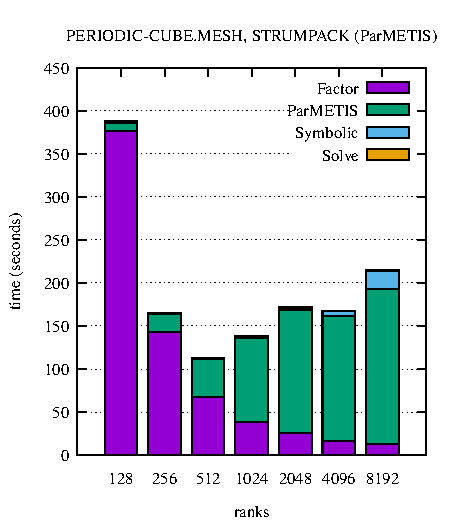
\includegraphics[scale=0.7]{projects/2.3.3-MathLibs/2.3.3.07-STRUMPACK-SuperLU/periodic-cube-scaling-strumpack.pdf}
\caption{STRUMPACK scaling with ParMETIS.}
\label{fig:strumpack-parmetis-scaling}
\end{minipage}
\begin{minipage}[b]{0.48\columnwidth}
\centering
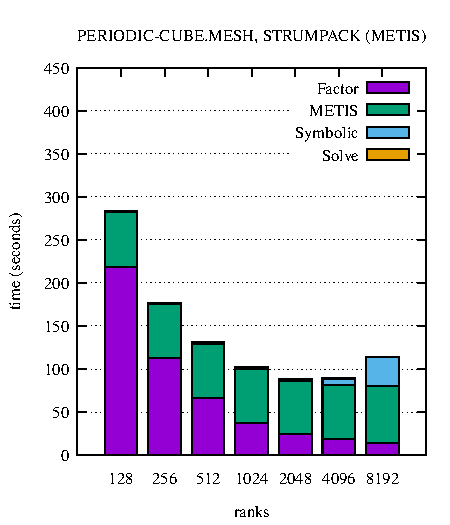
\includegraphics[scale=0.7]{projects/2.3.3-MathLibs/2.3.3.07-STRUMPACK-SuperLU/periodic-cube-scaling-strumpack_metis.pdf}
\caption{STRUMPACK scaling with METIS.}
\label{fig:strumpack-metis-scaling}
\end{minipage}
\end{figure}

\ignore{  %%%% from last period ....
\begin{enumerate}
\item We developed and evaluated a fully algebraic sparse preconditioner in 
      STRUMPACK. On top of the baseline multifrontal direct solver, we use
      low-rank compression in dense frontal matrices to obtain approximate
      factorization. We showed that our MF+HSS preconditioner is more robust
      for numerically hard problems than many alternatives. Our code
      strong scales to over 6000 cores~\cite{ghysels2017-ipdps}
      (Fig.~\ref{fig:strumpack-scaling}).
\item We developed several strategies to enhance scalability of triangular
      solve in SuperLU\_DIST. One is an asynchronous tree-based 
      broadcast/reduction scheme which reduces latency and improves
      communication load balance. Another is efficient threading implementation
      and BLAS operations. The new code is 4.4x and 6.1x faster on 4096 cores
      with one and 50 right-hand sides, respectively~\cite{LiuTriSolve2018}
      (Fig.~\ref{fig:superlu-trisolve}).
\item We developed a new communication-avoiding 3D sparse LU factorization
      (IPDPS) algorithm that has provably asymptotic lower communication
      complexity in both latency and volume. The prototype implementation
      in SuperLU\_DIST achieves up to 27x improvement over the baseline 
      2D algorithm when run on 24,000 cores of Edison at
      NERSC~\cite{sao2018}.
\item In collaboration with ExaGraph ECP project, we evaluated the performance
      of a parallel pre-ordering algorithm called Approximate-Weight Perfect
      Matching (AWPM) for pivot selection in SuperLU\_DIST. 
      For most practical problems (e.g.,DOE apps, and SuiteSparse) the 
      weights of the perfect matchings generated by AWPM often within 99\%
      of the optimum. The MPI+OpenMP implementation on Cori at NERSC scales          up to 256 nodes –-- 2500x faster than serial MC64, and up to 114x
      speedup on 256 nodes (17,408 cores) Cori-KNL~\cite{AWPM2018}.
      The interface to AWPM are already implemented in both STRUMPACK and
      SuperLU and are released.
\end{enumerate}
} %%%% ignored from last period ....


\paragraph{Next Steps} Our future efforts will focus on the following areas:
%\textit{Describe what you are working on next.}
\begin{itemize}
\item We will build detailed performance models and performance specific
  code optimizations for the ECP applications that use our solvers.
\item We will design and implement new algorithms for the GPU systems.
\end{itemize}

\ignore{  %%%% from last period ....
\begin{itemize}
\item For STRUMPACK, we will improve the performance of the HSS solve
      routine, add OpenMP and reduce communication. We will implement
      the HOLDR low-rank format.
\item For both STRUMPACK and SuperLU, we will build detailed performance
      models and performance specific code optimizations for the ECP
      applications that use our solvers.
\end{itemize}
} %%%% ignored from last period ....

%%%%%%%%%%%%%%%%%%%%%%%%%%%%%%%%%%%%%%%%%%%%%%%%%%%%
%%%% FFTX sub-project %%%%
%%%%%%%%%%%%%%%%%%%%%%%%%%%%%%%%%%%%%%%%%%%%%%%%%%%%
\subsubsection{\stid{3.07} Sub-project: FFTX} \label{subsubsect:fftx}
\noindent

\paragraph{Overview}
The use of FFTs span a broad range of DOE science applications, including ones represented in the Exascale applications space. Most applications use the API from FFTW, an open-source library developed in the 1990's. FFTW is still used extensively on DOE HPC platforms, and the FFTW API has become the de-facto
standard FFT interface: vendors that provide FFT libraries implement
(at least a subset) of that interface. Thus, FFTW both defines the 
standard FFT library interface, as well as being a key software component
for applications.
In the FFTX project, we are developing a new package for supporting FFT applications on exascale architectures. Our approach based on two ideas. The first is develop a backwards-compatible approach that builds on the FFTW interface but extends it to enable extraction of high performance on exascale machines. The second idea is to provide a toolchain that enables the
specialization of the FFT calculation and its surrounding use case calculations (scaling, data layout transformation, marshalling/unmarshalling for communication), using code generation, symbolic analysis, automatic performance tuning, and applications-specific code generation. We will use SPIRAL, an open-source toolchain for FFT developed at CMU, as the basis for developing FFTX, and will use specific ECP applications and target ECP exascale platforms to provide a focus for this work.

\paragraph{Key Challenges}
The traditional approach of of applications using FFTs is to build up high-performance implementations out of calls to (usually 1D) FFT libraries (either FFTW or vendor libraries), interleaved with user-implemented code for use-case-specific operations. This approach may break down on the emerging ECP platforms, for two reasons. The first is that the node architectures have become more complex. Multiple cores and accelerators lead to multiple levels of parallelism, including threading and SIMD/SIMT. In addition, there are on-node complex memory hierarchies that are to varying extents user-controlled, and across which it is expensive to move data. This leads to more complex interleaving of the other components of multidimensional FFT-based applications with the core library FFTs in order to maximize the effective use of the floating point capabilities and minimize data movement across the memory hierarchy. Some of these are simply not expressible in the current FFTW interface; others can be expressed, but with great effort on the part of the applications programmer, and often with an outcome of not yielding the theoretically-predicted performance due to unexpected and opaque behavior of the FFT library software. A second problem is that the open-source FFTW libraries are no longer supported. The original developers have gone on to other things, and the support of FFTW, such as it is, is performed by volunteer labor. As a result, the extensions to support new node architectures are more brittle and provide less coverage. Expanding the feature set of FFTW to enable the more effective use of the new node architectures is not feasible, since it would entail significant modification and use of the back-end software system, which no one is supporting, and on which the expertise is no longer available.

\paragraph{Solution Strategies} 
There are three components to our approach to providing a new software stack for FFT applications.

\begin{trivlist}
\item
(1) We will design an extension of the FFTW interface that both meets the needs of the FFT use cases arising in ECP applications, and exposes the
oppportunities for obtaining high performance on current and future 
architectures. The FFTX interface will be 
backwards compatible with FFTW so that legacy code using FFTW runs unmodified and gains substantially on hardware to which FFTX has been ported.
To express the additional opportunities for obtaining improved performance, we will add a small number of new features beyond the FFTW interface to express algorithmic features such as futures/delayed execution,
offloading, data placement, callback kernels, and sparsity of inputs or outputs. Such changes will have the potential to extract
much higher performance than standard FFTW calls, since higher level operations and new hardware features can be addressed. This interface will be designed as an embedded DSL, for which we will provide a standard C/C++ reference library implementation that enables rapid assessment of the interface by applications developers.
\item
(2) We will develop a new code-generation back end. FFT-based application kernels implemented using the extended FFTW interface described above will be treated as specifications. This allows the extraction of the algorithm semantics from source code and known library semantics, thus providing whole-kernel semantics and whole-kernel specifications. This enables build-time source-to-source translation and advanced performance optimizations, such as
cross-library optimization, targeting of accelerators through off-loading, and inlining of user-provided kernels.
Our approach allows for fine control over resource expenditure during optimization. Applications can control compile-time, initialization-time, invocation time optimization resources if they need to.
\item
(3) We will develop higher-level FFT-based applications driven primarily by the requirements of ECP applications projects, with the development of interfaces between FFTX and full ECP applications part of the co-design process. The strategy of having a library implementation of the FFTX interface will enable us to use the requirements of ECP applications for the design of the expanded FFTW interface and of the SPIRAL-based toolchain; in addition, the insights provided by opening up the design / tuning space for the constituent FFTs will lead to new ways of designing the applications solvers in order to obtain high performance. We will release the resulting integrated FFT-based packages as a library, called {\em SpectralPack}.

\end{trivlist}

The core code generation, symbolic analysis, and autotuning software for this project will be based on the open-source SPIRAL software stack,
building on 20 years of research by the SPIRAL team at CMU.
SPIRAL automatically maps computational kernels across a wide range of computing platforms to highly efficient code, and proves the correctness of the synthesized code.
The SPIRAL approach has many of the same structural components as FFTW -- a high-level DSL, symbolic analysis, code generation, and autotuning. However, the approach used by SPIRAL integrates these ideas more closely into the user code, generating new source code for both the FFT calls and the glue code (e.g. pointwise operations, data motion) in an FFT-based application.


